% Provenance (never printed): see sources/outline_sources.md (Year 3:
% fractionation and Rayleigh distillation in the water cycle;
% palaeothermometry; carbon and sulfur isotopes). Brief:
% sources/book5/BRIEFS.md, ch. 14. Curves from figdata/bachelor-3/
% rayleigh_distillation.py, lr04_d18o.py, carbon_mass_balance.py. Exercise
% and problem values in the Book 5 scratch calculator calc/ch14.py. Dome Ilse,
% its traverse and the marine core are invented.
\chapter{स्थायी-समस्थानिक भू-रसायन}\label{ch:b3:stable-isotopes}

पूर्वी अंटार्कटिक हिमचादर के ऊँचे गुंबदों पर गिरने वाला हिम पृथ्वी पर
सबसे हल्के जल में से एक है। इसका हर अणु वाष्प के रूप में महासागर से निकला था, और
अंतर्देशीय यात्रा में वायु ने अपना अधिकांश जल हिम के रूप में खो दिया, और भारी
अणु पहले गिरे। पहुँचने पर जो शेष रहता है, वह इस पर निर्भर करता है कि कितना
जल खोया गया, और यह इस पर निर्भर करता है कि वायु कितनी ठंडी हो गई। इसीलिए
बर्फ़ का एक स्तंभ एक तापमापी है, कैल्साइट का एक कवच दूसरा, और चूना-पत्थरों का
कार्बन जीवमंडल द्वारा दफ़न किए गए पदार्थ का एक लेखा-बही है। यह अध्याय इन
अभिलेखों के पीछे के नियम निकालता है और उन्हें पढ़ता है।

\begin{recall}
$\delta$ मान, प्रभाजन गुणांक $\alpha$ तथा साम्य और गतिक समस्थानिक
प्रभाव रसायन की पुस्तकों के विश्वविद्यालय खंडों में हैं। मानक VSMOW और VPDB
तथा उल्कीय जल रेखा पुस्तक 4 (स्नातक वर्ष 2) के समस्थानिक भू-रसायन वाले
अध्याय में हैं; मैग्मीय विभेदन वाले अध्याय में
अनुरेखी तत्त्वों का रैले प्रभाजन नियम है;
जलवायु अभिलेखागार और प्रॉक्सी वाले अध्याय में हिम-आयतन प्रभाव और Mg/Ca
तापमापी हैं; भूवैज्ञानिक समय में जलवायु वाले अध्याय में पैलियोसीन--इओसीन
ऊष्मीय अधिकतम है; पृथ्वी के प्रीकैम्ब्रियन काल वाले अध्याय में महा ऑक्सीकरण
घटना है।
प्रकाश-संश्लेषण और जीवाणु सल्फ़ेट अपचयन जीवविज्ञान की पुस्तकों में हैं।
\end{recall}

\section{दो प्रावस्थाओं के बीच प्रभाजन}\label{sec:b3:stable-isotopes:fractionation}

समस्थानिक साम्य में स्थित दो प्रावस्थाओं A और B के लिए $\alpha_{A-B} = R_A/R_B =
(1000 + \delta_A)/(1000 + \delta_B)$, जहाँ $R$ भारी और हल्के समस्थानिक का अनुपात है।
जलवाष्प और द्रव जल के लिए ऑक्सीजन-18 हेतु $\alpha = 1.0098$ और
ड्यूटेरियम हेतु \qty{20}{\celsius} पर $1.084$ है; \qty{0}{\celsius} पर क्रमशः
$1.0117$ और $1.111$ है; बर्फ़ और जल के लिए \qty{0}{\celsius} पर $1.0035$ और $1.0208$ है।
भारी प्रावस्था सदा अधिक संघनित होती है, और
तापमान गिरने के साथ प्रभाजन बढ़ता है।
% ledger: kc98:alpha, kc98:standards

\begin{definition}[समस्थानिक अंतर]\label{def:b3:stable-isotopes:big-delta}
दो प्रावस्थाओं के बीच \emph{समस्थानिक अंतर}\index{समस्थानिक अंतर (बड़ा डेल्टा)}
$\Delta_{A-B} = \delta_A - \delta_B$ है, प्रति मिल में।
\end{definition}

\begin{proposition}[समस्थानिक अंतर और प्रभाजन गुणांक]
\label{prop:b3:stable-isotopes:big-delta}
जब $\alpha$ 1 के निकट और $\delta$ मान छोटे हों,
\[
\Delta_{A-B} \approx 1000\ln\alpha_{A-B} \approx 1000(\alpha_{A-B} - 1).
\]
\end{proposition}

\begin{proof}
$1000\ln\alpha = 1000\ln(1 + \delta_A/1000) - 1000\ln(1 + \delta_B/1000)$, और
$1000\ln(1 + x/1000) = x - x^2/2000 + \dots$, अतः $1000\ln\alpha = \delta_A -
\delta_B - (\delta_A^2 - \delta_B^2)/2000 + \dots$। अंततः $\ln\alpha \approx
\alpha - 1$ होता है, जब $\alpha$ 1 के निकट हो।
\end{proof}

त्रुटि $(\delta_A^2 - \delta_B^2)/2000$ है: महासागर के मानों पर प्रति मिल का एक भाग,
और महासागर तथा ध्रुवीय बर्फ़ के हल्के हिम के बीच लगभग एक
प्रति मिल।
सिद्धांत जिस राशि को तापमान से जोड़ता है, वह $1000\ln\alpha$ है: वह
उच्च तापमान पर लगभग $1/T^2$ के अनुसार और निम्न तापमान पर $1/T$ के अनुसार बदलती है,
और अंशांकन इसी रूप में लिखे जाते हैं। उदाहरण के लिए बर्फ़ और वाष्प के लिए
\[
\ln\alpha^{18}_{\mathrm{ice-v}} = \frac{11.839}{T} - 0.028224, \qquad
\ln\alpha^{\mathrm D}_{\mathrm{ice-v}} = \frac{16288}{T^2} - 0.0934,
\]
जहाँ $T$ केल्विन में है।
% ledger: gkinis14:alpha-ice, kc98:standards

\begin{definition}[द्रव्यमान-आश्रित और द्रव्यमान-स्वतंत्र प्रभाजन]\label{def:b3:stable-isotopes:mif}
तीन या अधिक समस्थानिकों वाले तत्त्व में \emph{द्रव्यमान-आश्रित
प्रभाजन}\index{द्रव्यमान-आश्रित प्रभाजन} तब होता है जब उसके समस्थानिक अनुपातों के प्रभाजन
उनके द्रव्यमान अंतरों के अनुपात में हों, जैसा द्रव्यमानों द्वारा तय होता है;
अन्यथा उसमें \emph{द्रव्यमान-स्वतंत्र
प्रभाजन}\index{द्रव्यमान-स्वतंत्र प्रभाजन} होता है, जिसे द्रव्यमान-आश्रित रेखा से
विचलन से मापा जाता है, जैसे $\Delta^{33}\mathrm S = \delta^{33}\mathrm S
- 0.515\,\delta^{34}\mathrm S$।
\end{definition}

ऑक्सीजन के लिए $^{17}\mathrm O/^{16}\mathrm O$ का प्रभाजन $^{18}\mathrm O/^{16}\mathrm O$ के
लगभग 0.52 गुना है, जो द्रव्यमान अंतरों के अनुपात, 1 से 2, के निकट है;
सल्फ़र के लिए $\delta^{33}\mathrm S = 0.515\,\delta^{34}\mathrm S$ है।
\omterm{def:b3:stable-isotopes:mif}{द्रव्यमान-स्वतंत्र प्रभाजन} दुर्लभ है: यह उल्कापिंडों, समताप मंडल की ओज़ोन और
आर्कियन सल्फ़र में पाया जाता है।
% ledger: white13c9:mdf, white13c9:s-mif

\section{जल चक्र में रैले आसवन}\label{sec:b3:stable-isotopes:rayleigh}

ठंडी होती वायु राशि बादल की बूँदें या हिम के क्रिस्टल बनाती है, जो गिरकर
निकल जाते हैं। हर संघनित पदार्थ वाष्प से भारी समस्थानिकों में अधिक समृद्ध होता है,
इसलिए शेष बची वाष्प और हल्की होती जाती है, और उसके साथ साम्य में बना अगला संघनित पदार्थ
भी और हल्का होता है।

\begin{proposition}[रैले आसवन]\label{prop:b3:stable-isotopes:rayleigh-distillation}
मान लीजिए वाष्प का एक भंडार संघनित पदार्थों द्वारा अपना जल खोता है, जिनमें से
हर एक वाष्प के साथ साम्य में बनते ही हटा दिया जाता है। यदि $f$ शेष बची
वाष्प का भाग है और $\alpha$ संघनित पदार्थ--वाष्प प्रभाजन गुणांक है, तो
वाष्प का अनुपात $\mathrm d\ln R_v = (\alpha - 1)\,\mathrm d\ln f$ का पालन करता है। स्थिर
$\alpha$ के लिए यह \emph{रैले
आसवन}\index{रैले आसवन}:
\[
\frac{R_v}{R_{v,0}} = f^{\,\alpha - 1}, \qquad
\delta_v = (1000 + \delta_{v,0})\,f^{\,\alpha - 1} - 1000,
\]
और $f$ पर बने संघनित पदार्थ का $\delta_c = \alpha(1000 + \delta_v) - 1000$ है।
\end{proposition}

\begin{proof}
मान लीजिए $N$ जलवाष्प के अणुओं की संख्या है (लगभग सभी हल्के) और $N R_v$
भारी अणुओं की संख्या है। संघनित पदार्थ के $\mathrm dN < 0$ अणु हटाने से
$\alpha R_v\,\mathrm dN$ भारी अणु हट जाते हैं: $\mathrm d(NR_v) = \alpha
R_v\,\mathrm dN$। अतः $N\,\mathrm dR_v = (\alpha - 1)R_v\,\mathrm dN$ प्राप्त होता है, जो
$f = N/N_0$ के साथ अवकलीय नियम है। स्थिर $\alpha$ के लिए यह समाकलित होकर
घात नियम बन जाता है।
\end{proof}

जब $\alpha$ तापमान पर निर्भर हो, तब $\ln(R_v/R_{v,0}) = \int(\alpha - 1)\,
\mathrm d\ln f$ मार्ग के साथ होता है। स्थिर दाब पर ठंडी होती वायु राशि के लिए,
वह जितना जलवाष्प धारण कर सकती है, वह संतृप्ति दाब से तय होता है, इसलिए $f =
e_s(T)/e_s(T_0)$ होता है, जिसे बर्फ़ का उर्ध्वपातन वक्र
\qty{0}{\celsius} से नीचे देता है। नीचे का चित्र उस वायु राशि के लिए नियम का समाकलन करता है
जिसका जलवाष्प \qty{0}{\celsius} से आरंभ होता है, और जिसका माना गया $\delta^{18}\mathrm O = -20$
और $\delta\mathrm D = \qty{-150}{\permil}$ है। महासागर के ऊपर का वास्तविक जलवाष्प
समुद्री जल के साथ साम्य उसे जितना बनाता, उससे हल्का होता है। ऑक्सीजन-18 में यह लगभग $-13$ है,
\qty{-9}{\permil} के बजाय, क्योंकि वाष्पीकरण आंशिक रूप से गतिक होता है।
% ledger: iapws:melt-subl, gkinis14:alpha-ice, white13c9:rayleigh

\begin{definition}[ड्यूटेरियम आधिक्य]\label{def:b3:stable-isotopes:d-excess}
\emph{ड्यूटेरियम आधिक्य}\index{ड्यूटेरियम आधिक्य} किसी जल नमूने का $d =
\delta\mathrm D - 8\,\delta^{18}\mathrm O$ होता है, प्रति मिल में।
\end{definition}

उत्तरी गोलार्ध के महाद्वीपों से होने वाला वर्षण
$\delta\mathrm D = 8.0\,\delta^{18}\mathrm O + 10$ रेखा पर स्थित होता है: इसका \omterm{def:b3:stable-isotopes:d-excess}{ड्यूटेरियम आधिक्य} लगभग
\qty{10}{\permil} है। ढलान 8 संघनन में दोनों समस्थानिकों के साम्य
प्रभाजनों के अनुपात के निकट है। 10 का आधिक्य, 0 नहीं,
महासागर से होने वाले गतिक वाष्पीकरण को दर्ज करता है, और किसी नमूने का आधिक्य
बताता है कि उसका जल साम्य से कितनी दूर तक वाष्पित हुआ।
% ledger: dansgaard64:effects, kc98:mwl

\begin{omfigure}
\begin{tikzpicture}
\begin{groupplot}[group style={group size=2 by 1, horizontal sep=1.6cm},
  omrecord, width=0.47\linewidth, height=0.42\linewidth, title style={font=\small},
  tick label style={font=\scriptsize}, label style={font=\small},
  legend style={font=\scriptsize, legend cell align=left}]
\nextgroupplot[title={(क) शीतलन मार्ग के साथ},
  xlabel={संघनन तापमान (\unit{\celsius})}, ylabel={$\delta^{18}\mathrm O$ (\unit{\permil})},
  xmin=-55, xmax=0, ymin=-130, ymax=0, x dir=reverse,
  legend style={at={(0.03,0.03)}, anchor=south west}]
% computed in figdata/bachelor-3/rayleigh_distillation.py
\addplot[omDef, thick, densely dashed] table[x=t, y=d18v] {figdata/out/bachelor-3-rayleigh_distillation-curve.dat};
\addlegendentry{जलवाष्प}
\addplot[omDef, thick] table[x=t, y=d18s] {figdata/out/bachelor-3-rayleigh_distillation-curve.dat};
\addlegendentry{हिम}
\addplot[red!70!black, only marks, mark=*, mark size=1.6pt] table[x=t, y=d18s] {figdata/out/bachelor-3-rayleigh_distillation-stations.dat};
\addlegendentry{केंद्र}
\nextgroupplot[title={(ख) $\delta\mathrm D$--$\delta^{18}\mathrm O$ आलेख पर हिम},
  xlabel={$\delta^{18}\mathrm O$ (\unit{\permil})}, ylabel={$\delta\mathrm D$ (\unit{\permil})},
  xmin=-110, xmax=0, ymin=-700, ymax=0,
  legend style={at={(0.97,0.03)}, anchor=south east}]
\addplot[omDef, thick] table[x=d18s, y=dDs] {figdata/out/bachelor-3-rayleigh_distillation-curve.dat};
\addlegendentry{मॉडल हिम}
\addplot[black, densely dotted, domain=-110:0, samples=2] {8*x + 10};
\addlegendentry{$\delta\mathrm D = 8\,\delta^{18}\mathrm O + 10$}
\addplot[red!70!black, only marks, mark=*, mark size=1.6pt, forget plot] table[x=d18s, y=dDs] {figdata/out/bachelor-3-rayleigh_distillation-stations.dat};
\end{groupplot}
\end{tikzpicture}

\par\smallskip{\small स्थिर दाब पर \qty{0}{\celsius} से ठंडी होती वायु राशि का \omterm{prop:b3:stable-isotopes:rayleigh-distillation}{रैले आसवन},
जिसमें बर्फ़-वाष्प प्रभाजन गुणांक और बचे जलवाष्प का अंश
बर्फ़ के उर्ध्वपातन वक्र से पढ़े गए हैं। (क)
जलवाष्प (टूटी रेखा) और हिम (ठोस रेखा) अधिकाधिक तेज़ी से हल्के होते जाते हैं; बिंदु
सप्ताहांत समस्या के तीन केंद्र हैं। (ख) मॉडल हिम ऑक्सीजन-18 में लगभग
\qty{-30}{\permil} तक उल्कीय जल रेखा के निकट रहता है, फिर
उससे ऊपर उठता है।}\label{fig:b3:stable-isotopes:rayleigh}
\end{omfigure}
% ledger: kc98:mwl


\begin{definition}[तापमान, मात्रा और महाद्वीपीय प्रभाव]\label{def:b3:stable-isotopes:effects}
\emph{तापमान प्रभाव}\index{तापमान प्रभाव (समस्थानिक)} वर्षण के
$\delta^{18}\mathrm O$ और $\delta\mathrm D$ की स्थानीय तापमान के साथ होने वाली कमी है।
\emph{मात्रा प्रभाव}\index{मात्रा प्रभाव} उष्णकटिबंधों में वर्षा की मात्रा के साथ
उनकी कमी है। \emph{महाद्वीपीय
प्रभाव}\index{महाद्वीपीय प्रभाव} अंतर्देशीय क्षेत्रों में
दिए गए तापमान पर उनकी कमी है।
\end{definition}

ये तीनों भूतल से देखे गए \omterm{prop:b3:stable-isotopes:rayleigh-distillation}{रैले आसवन} ही हैं। उच्च अक्षांशों पर
\omterm{def:b3:stable-isotopes:effects}{तापमान प्रभाव} प्रमुख होता है: ग्रीनलैंड और उत्तरी अटलांटिक के केंद्रों के वार्षिक माध्य
$\delta^{18}\mathrm O = 0.69\,t - 13.6$ और $\delta\mathrm D =
5.6\,t - 100$ का अनुसरण करते हैं (प्रति मिल में, जहाँ $t$ वार्षिक माध्य भूतलीय तापमान है,
\unit{\celsius} में)। उष्णकटिबंधों में \omterm{def:b3:stable-isotopes:effects}{मात्रा प्रभाव} प्रमुख होता है: एक महासागरीय द्वीप पर,
मासिक वर्षा में ऑक्सीजन-18 लगभग \qty{1.6}{\permil} घटती है, हर
\qty{100}{mm} अधिक वर्षा पर। ऊपर के चित्र का सरल मॉडल इससे अधिक तीखी ढलान देता है,
जो संघनन तापमान के प्रति डिग्री लगभग \qty{1.6}{\permil} है। इन ढलानों की प्रत्यक्ष तुलना
नहीं हो सकती: हिमचादर का पृष्ठ ठंडा होता है
उस वायु से जहाँ हिम बनता है, और मॉडल वायु राशियों के मिश्रण
तथा हिम-निर्माण के गतिक प्रभावों को अनदेखा करता है, इसलिए भूतलीय तापमान के विरुद्ध
ढलान परिकलित नहीं, बल्कि अंशांकित है।
% ledger: dansgaard64:effects

\section{पुरा-तापमिति}\label{sec:b3:stable-isotopes:palaeothermometry}

\begin{definition}[पुरा-तापमिति, पुरा-तापमान समीकरण]
\label{def:b3:stable-isotopes:palaeothermometry}
\emph{पुरा-तापमिति}\index{पुरा-तापमिति} उन पदार्थों की संरचना से अतीत के
तापमानों का मापन है, जो तब बने थे। एक
\emph{पुरा-तापमान समीकरण}\index{पुरा-तापमान समीकरण} एक
अंशांकित संबंध है, जो किसी खनिज के निर्माण के तापमान और
जिस जल से वह उगा था, उसके साथ उसके प्रभाजन के बीच होता है।
\end{definition}

जल से धीरे-धीरे अवक्षेपित कैल्साइट के लिए एक अंशांकन यह देता है
\[
1000\ln\alpha_{\mathrm{calcite-water}} = 18.03\,\frac{10^3}{T} - 32.42,
\]
दोनों $\delta$ मान VSMOW पैमाने पर हैं। कार्बोनेट VPDB पैमाने पर दर्ज होते हैं,
जिन्हें $\delta^{18}\mathrm O_{\mathrm{VPDB}} =
0.97001\,\delta^{18}\mathrm O_{\mathrm{VSMOW}} - 29.99$ से बदला जाता है। \qty{5}{\celsius} के निकट
प्रभाजन प्रति डिग्री तापन पर लगभग \qty{0.23}{\permil} घटता है।
% ledger: isogeochem:ko97

\begin{method}[कार्बोनेट पुरा-तापमान]\label{met:b3:stable-isotopes:palaeotemperature}
\begin{enumerate}
\item कैल्साइट के $\delta^{18}\mathrm O$ को VPDB से VSMOW में बदलिए;
\item जिस जल से कवच बना, उसके $\delta^{18}\mathrm O$ का अनुमान
VSMOW पर लगाइए, वर्तमान मान को उस समय के हिम-आयतन के लिए संशोधित करते हुए;
\item $1000\ln\alpha = 1000\ln[(1000 + \delta_c)/(1000 + \delta_w)]$ परिकलित कीजिए;
\item अंशांकन को उलटिए: $T = 18.03\times10^3/(1000\ln\alpha + 32.42)$।
\end{enumerate}
\end{method}

दूसरा चरण कठिन है। हिमनदीकरण के दौरान हिमचादरें
हल्का जल संचित कर लेती हैं, और महासागर अधिक भारी होता जाता है। समुद्र-तल का प्रत्येक मीटर
महासागर के $\delta^{18}\mathrm O$ में लगभग \qty{0.011}{\permil} के अनुरूप होता है; अंतिम हिमनदीय
काल में समुद्र-तल लगभग \qty{125}{m} घटा, जिससे महासागर लगभग
\qty{1.4}{\permil} भारी हो गया। जीव अपने स्वयं के विचलन जोड़ते हैं, जिन्हें
जैविक प्रभाव कहते हैं, और दफ़न के बाद कवच छिद्र-जल से ऑक्सीजन का विनिमय कर सकता है।
% ledger: white13c9:ice-volume

\begin{omfigure}
\begin{tikzpicture}
\begin{axis}[omrecord, width=0.8\linewidth, height=0.32\linewidth, clip=false,
  xlabel={आयु (\unit{\ka})}, ylabel={तलीय $\delta^{18}\mathrm O$ (\unit{\permil})},
  xmin=0, xmax=800, ymin=2.8, ymax=5.4, y dir=reverse,
  xtick={0,100,200,300,400,500,600,700,800},
  tick label style={font=\scriptsize}, label style={font=\small}]
% computed in figdata/bachelor-3/lr04_d18o.py from data/derived/lr04.csv
\addplot[omDef, thin] table[x=age_ka, y=d18O] {figdata/out/bachelor-3-lr04_d18o-stack.dat};
\draw[densely dotted] (axis cs:0,3.25) -- (axis cs:830,3.25);
\draw[densely dotted] (axis cs:20,5.02) -- (axis cs:830,5.02);
\draw[red!70!black, thick, |-|] (axis cs:830,3.25) -- node[right, font=\scriptsize, align=left] {हिम-आयतन\\\qty{1.4}{\permil}} (axis cs:830,4.625);
\draw[black, thick, |-|] (axis cs:830,4.625) -- node[right, font=\scriptsize] {शीतलन} (axis cs:830,5.02);
\end{axis}
\end{tikzpicture}

\par\smallskip{\small वैश्विक स्टैकिंग, जो तलीय फ़ोरामिनिफ़र के $\delta^{18}\mathrm O$ का है,
पिछले \qty{800}{\ka} में, अक्ष उलटा है ताकि ठंडे हिमनदीय काल
नीचे दिखें। वर्तमान (\qty{3.25}{\permil}) से अंतिम हिमनदीय अधिकतम
(\qty{5.02}{\permil}) तक लगभग \qty{1.4}{\permil} का परिवर्तन हिम-आयतन का है (लाल पट्टी, दाईं ओर);
शेष परिवर्तन गहरे जल के शीतलन का है (काली
पट्टी)।}\label{fig:b3:stable-isotopes:lr04}
\end{omfigure}
% ledger: data:lr04, white13c9:ice-volume

\begin{definition}[गुच्छित समस्थानिक]\label{def:b3:stable-isotopes:clumped}
\emph{गुच्छित समस्थानिक}\index{गुच्छित समस्थानिक} वे अणु या समूह हैं जिनमें
दो भारी समस्थानिक आपस में जुड़े होते हैं। कार्बोनेटों में $\Delta_{47}$ वह
आधिक्य है, प्रति मिल में, $^{13}\mathrm C^{18}\mathrm O^{16}\mathrm O_2$ समूहों की बहुतायत का,
जो द्रव्यमान-47 कार्बन डाइऑक्साइड के रूप में मापा जाता है, समस्थानिकों के यादृच्छिक
वितरण की तुलना में।
\end{definition}

भारी समस्थानिक संयोग की अपेक्षा कुछ अधिक आपस में जुड़ते हैं,
और क्रिस्टल जितना ठंडा होगा, उतना ही अधिक। आधिक्य केवल
वृद्धि के तापमान पर निर्भर करता है, जल की संरचना पर नहीं; एक एकीकृत
अंशांकन है $\Delta_{47} = 0.0391\times10^6/T^2 + 0.154$ (प्रति मिल में, $T$
केल्विन में) 0.5 से \qty{1100}{\celsius} तक। इसे
$\delta^{18}\mathrm O$ के साथ मापने पर यह तापमान और
जल की संरचना, दोनों देता है। इसकी संवेदनशीलता छोटी है, प्रति डिग्री लगभग \qty{0.003}{\permil}, जो
\qty{20}{\celsius} के निकट है, इसलिए लंबे मापन आवश्यक होते हैं।
% ledger: isogeochem:d47

\section{कार्बन समस्थानिक}\label{sec:b3:stable-isotopes:carbon}

प्रकाश-संश्लेषण गतिकीय रूप से कार्बन का प्रभाजन करता है। कार्बन
डाइऑक्साइड का पत्ती में विसरण लगभग \qty{-4.4}{\permil} का, और एंज़ाइम RuBisCO
\qty{-29.4}{\permil} का प्रभाव डालता है; सामान्य C3 मार्ग के पौधे वायु से \num{20} से
\qty{30}{\permil} तक हल्के होते हैं, और औसतन लगभग
\qty{-27}{\permil} होते हैं, जबकि C4 मार्ग के पौधे लगभग \qty{-13}{\permil}। जैविक
कार्बन हल्का होता है, और जिस अकार्बनिक कार्बन से वह बनता है, वह भारी होता जाता है।
% ledger: white13c9:photosynthesis, white:d13c

\begin{definition}[कार्बनिक कार्बन दफ़न अंश]\label{def:b3:stable-isotopes:forg}
\emph{कार्बनिक कार्बन दफ़न अंश}\index{कार्बनिक कार्बन दफ़न अंश}
$f_{\mathrm{org}}$ वह अंश है जो महासागर और वायुमंडल से निकलने वाले
कार्बन में से कार्बोनेट के बजाय कार्बनिक पदार्थ के रूप में दफ़न होता है।
\end{definition}

\begin{proposition}[कार्बन समस्थानिक द्रव्यमान संतुलन]\label{prop:b3:stable-isotopes:forg}
स्थायी अवस्था में, संघटन $\delta_{\mathrm{in}}$ वाले आगत और कार्बोनेट का दफ़न
$\delta_{\mathrm{carb}}$ तथा कार्बनिक कार्बन का दफ़न $\delta_{\mathrm{org}} =
\delta_{\mathrm{carb}} + \Delta_B$ होने पर, \emph{कार्बन समस्थानिक
द्रव्यमान संतुलन}\index{कार्बन समस्थानिक द्रव्यमान संतुलन} निम्नलिखित है
\[
\delta_{\mathrm{in}} = f_{\mathrm{org}}\,\delta_{\mathrm{org}} + (1 - f_{\mathrm{org}})\,
\delta_{\mathrm{carb}}, \qquad f_{\mathrm{org}} = \frac{\delta_{\mathrm{in}} -
\delta_{\mathrm{carb}}}{\Delta_B}.
\]
\end{proposition}

\begin{proof}
स्थायी अवस्था में प्रवेश करने वाला कार्बन उतना ही होता है जितना दफ़न होने वाला, और कार्बन-13 के लिए भी यही सच है; $\delta$ मानों के साथ कार्बन-13 का संतुलन द्रव्यमान-भारित
माध्य होता है, जो $\delta$ मानों पर लागू होता है और
\cref{prop:b3:stable-isotopes:big-delta} के सन्निकटन तक मान्य है।
$\delta_{\mathrm{org}} =
\delta_{\mathrm{carb}} + \Delta_B$ रखने और हल करने पर $f_{\mathrm{org}}$ प्राप्त होता है।
\end{proof}

आगत, जो ज्वालामुखियों से और पुराने कार्बोनेटों तथा कार्बनिक
पदार्थ के अपक्षय से आते हैं, लगभग \qty{-5}{\permil} माने जाते हैं, जो प्रावार का मान है; $\Delta_B$
$-32$ और \qty{-25}{\permil} के बीच रहा है; और कार्बोनेटों ने
$\delta^{13}\mathrm C$ को लगभग 0 के निकट, लगभग \qty{1}{\permil} के भीतर, पृथ्वी के इतिहास के अधिकांश
भाग में बनाए रखा है। संतुलन तब शास्त्रीय $f_{\mathrm{org}} \approx
0.2$ प्राप्त होता है: कार्बन का पाँचवाँ भाग कार्बनिक पदार्थ के रूप में दफ़न होता है, और उसके साथ
प्रकाश-संश्लेषण से मुक्त हुई ऑक्सीजन वायुमंडल में बनी रहती है। हाल का कार्य तर्क देता है कि
$f_{\mathrm{org}}$ इस स्थिरता के सुझाव से कहीं अधिक बदला है।
% ledger: planavsky22:forg

\begin{definition}[कार्बन समस्थानिक विचलन]\label{def:b3:stable-isotopes:cie}
\emph{कार्बन समस्थानिक विचलन}\index{कार्बन समस्थानिक विचलन} एक
भूवैज्ञानिक रूप से संक्षिप्त बदलाव है, जो कार्बोनेटों और कार्बनिक
पदार्थ के $\delta^{13}\mathrm C$ में विश्वव्यापी होता है, जिसके बाद वापसी होती है और जो अवसादी अनुक्रमों में दर्ज होती है।
\end{definition}

\begin{proposition}[विचलन का द्रव्यमान]\label{prop:b3:stable-isotopes:cie-mass}
संघटन $\delta_s$ और द्रव्यमान $m$ वाला कार्बन,
द्रव्यमान $M$ और संघटन $\delta_0$ वाले विनिमेय भंडार में मिलाया जाए, तो वह उसे $\Delta$ से विचलित करता है, जब
\[
m = M\,\frac{\Delta}{\delta_s - \delta_0 - \Delta}.
\]
\end{proposition}

\begin{proof}
मिश्रण का $(M + m)(\delta_0 + \Delta) = M\delta_0 + m\delta_s$ होता है, जो
$m$ में रैखिक है।
\end{proof}

पैलियोसीन--इओसीन ऊष्मीय अधिकतम के आरंभ में, 55.5 और
\qty{56.3}{\Ma} के बीच, महासागर और वायुमंडल का कार्बन 2.5 से
\qty{4.0}{\permil} गिर गया, \qty{60}{kyr} से कम समय में। आवश्यक कार्बन लगभग
2000 से \qty{3500}{Gt} है, यदि यह \qty{-60}{\permil} पर मीथेन था, 6000 से
\qty{12000}{Gt}, यदि यह \qty{-25}{\permil} पर कार्बनिक कार्बन था: स्रोत जितना हल्का
होगा, उतना कम कार्बन चाहिए। पीछे की ओर पढ़ने पर
इस प्रतिज्ञप्ति के साथ और $\delta_0 = 0$ लेने पर, ये अनुमान विनिमेय भंडार में \num{46000}
से \qty{63000}{Gt} कार्बन का संकेत देते हैं।
% ledger: dickens11:petm

\begin{omfigure}
\begin{tikzpicture}
\begin{groupplot}[group style={group size=2 by 1, horizontal sep=1.7cm},
  omrecord, width=0.47\linewidth, height=0.4\linewidth, title style={font=\small},
  tick label style={font=\scriptsize}, label style={font=\small},
  legend style={font=\scriptsize, legend cell align=left}]
\nextgroupplot[title={(क) स्थायी अवस्था, $\delta_{\mathrm{in}} = \qty{-5}{\permil}$},
  xlabel={$f_{\mathrm{org}}$}, ylabel={$\delta^{13}\mathrm C_{\mathrm{carb}}$ (\unit{\permil})},
  xmin=0, xmax=0.4, ymin=-6, ymax=8, xtick={0,0.1,0.2,0.3,0.4}, xticklabels={0,0.1,0.2,0.3,0.4},
  legend style={at={(0.03,0.97)}, anchor=north west}]
% computed in figdata/bachelor-3/carbon_mass_balance.py
\addplot[omDef, thick] table[x=f, y=dcarb25] {figdata/out/bachelor-3-carbon_mass_balance-forg.dat};
\addlegendentry{$\Delta_B = \qty{-25}{\permil}$}
\addplot[red!70!black, thick] table[x=f, y=dcarb30] {figdata/out/bachelor-3-carbon_mass_balance-forg.dat};
\addlegendentry{$\Delta_B = \qty{-30}{\permil}$}
\nextgroupplot[title={(ख) विचलन के लिए कार्बन},
  xlabel={स्रोत का $\delta^{13}\mathrm C$ (\unit{\permil})}, ylabel={जोड़ा गया कार्बन (\unit{Gt})},
  xmin=-70, xmax=-20, ymin=0, ymax=14000, scaled y ticks=false,
  ytick={0,4000,8000,12000}, yticklabels={0,4000,8000,12000},
  legend style={at={(0.03,0.97)}, anchor=north west}]
\addplot[omDef, thick] table[x=ds, y=m25] {figdata/out/bachelor-3-carbon_mass_balance-mass.dat};
\addlegendentry{$\Delta = \qty{-2.5}{\permil}$}
\addplot[red!70!black, thick] table[x=ds, y=m40] {figdata/out/bachelor-3-carbon_mass_balance-mass.dat};
\addlegendentry{$\Delta = \qty{-4.0}{\permil}$}
\end{groupplot}
\end{tikzpicture}

\par\smallskip{\small (क) स्थायी अवस्था में दफ़न कार्बोनेट का $\delta^{13}\mathrm C$,
\omterm{def:b3:stable-isotopes:forg}{कार्बनिक कार्बन दफ़न अंश} के विरुद्ध: 0 के पास के कार्बोनेट का अर्थ है
$f_{\mathrm{org}}$ लगभग 0.2। (ख) 2.5 या
\qty{4.0}{\permil} के विचलन के लिए विनिमेय भंडार में
\qty{50000}{Gt} के, 0 पर, आवश्यक कार्बन, स्रोत के संघटन के विरुद्ध।}\label{fig:b3:stable-isotopes:carbon}
\end{omfigure}

\section{गंधक और वायु की ऑक्सीजन}\label{sec:b3:stable-isotopes:sulfur}

जीवाणुओं द्वारा सल्फेट अपचयन हल्का सल्फ़ाइड बनाता है, और इसके सभी प्रभाजन
द्रव्यमान-आश्रित होते हैं। आर्कियन अवसादी सल्फ़ाइड और सल्फ़ेट वह करते हैं जो कोई
नई चट्टान नहीं करती: \qty{2.45}{\Ga} से पहले उनका $\Delta^{33}\mathrm S$
\qty{3.5}{\permil} तक पहुँचता है; 2.45 और \qty{2.0}{\Ga} के बीच यह
\qty{0.5}{\permil} से नीचे रहता है; \qty{2.0}{\Ga} के बाद यह लुप्त हो जाता है। प्रयोगशाला में
पराबैंगनी प्रकाश, जो सल्फ़र डाइऑक्साइड को तोड़ता है, द्रव्यमान-स्वतंत्र गंधक बनाता है।
वायु में ऑक्सीजन और ओज़ोन न होने पर पराबैंगनी प्रकाश निचले
वायुमंडल तक पहुँचता था और ज्वालामुखीय सल्फ़र डाइऑक्साइड को विभाजित करता था; उत्पाद,
सल्फेट, जो ऋणात्मक है, और मूल गंधक, जो धनात्मक $\Delta^{33}\mathrm S$ वाला है, अलग-अलग
अवसादों तक पहुँचे। ऑक्सीजन बढ़ने पर ओज़ोन की ढाल ने प्रकाश-अपघटन को
रोक दिया, और उत्पादों के ऑक्सीकरण ने उन्हें फिर से मिला दिया। संकेत का
लुप्त होना वायुमंडलीय ऑक्सीजन के उदय के सबसे तीखे अभिलेखों में से एक है,
जिसे अन्य साक्ष्य लगभग 2 से \qty{2.3}{\Ga}
पहले रखते हैं।
% ledger: white13c9:s-mif

\begin{omfigure}
\begin{tikzpicture}[scale=0.9]
\draw[->] (0,0) -- (6,0);
\node[font=\small] at (3,-0.75) {$\delta^{34}\mathrm S$ (\unit{\permil})};
\draw[->] (0,0) -- (0,4) node[above, font=\small] {$\delta^{33}\mathrm S$ (\unit{\permil})};
\draw[omDef, thick] (0,0) -- (5.5,2.833) node[right, font=\scriptsize] {ढलान 0.515};
\fill[red!70!black] (3.0,3.05) circle (2pt) node[above left, font=\scriptsize] {आर्कियन पाइराइट};
\draw[<->, red!70!black] (3.0,1.545) -- node[right, font=\scriptsize] {$\Delta^{33}\mathrm S$} (3.0,2.95);
\fill[black] (4.0,2.06) circle (2pt) node[below right, font=\scriptsize] {नया सल्फ़ाइड};
\foreach \x in {1,2,3,4,5} \draw (\x,0) -- (\x,-0.08) node[below, font=\scriptsize] {\x};
\foreach \y in {1,2,3} \draw (0,\y) -- (-0.08,\y) node[left, font=\scriptsize] {\y};
\end{tikzpicture}

\par\smallskip{\small योजनाबद्ध तीन-समस्थानिक आलेख (प्रति मिल में एक इकाई)।
\omterm{def:b3:stable-isotopes:mif}{द्रव्यमान-आश्रित प्रभाजन} हर नमूने को 0.515 ढलान की एक रेखा पर रखता है; एक
आर्कियन पाइराइट, जिसका $\Delta^{33}\mathrm S = \qty{1.5}{\permil}$ है, उसके ऊपर स्थित है।}\label{fig:b3:stable-isotopes:three-isotope}
\end{omfigure}
% ledger: white13c9:s-mif

\begin{inthelab}[बर्फ़ के कोर से तापमान तक]
\begin{minipage}[t]{0.55\linewidth}\vspace{0pt}
हिमचादर पर एक ड्रिलिंग तंबू में कोर को मापा, दर्ज किया और लंबाइयों में
काटा जाता है, जैसे ही वह ऊपर आता है। प्रयोगशाला में एक नमूना-रेखा उसे एक सिरे से
लगातार पिघलाती है, और पिघला जल एक ऐसे उपकरण तक बहता है, जो
हर कुछ सेंटीमीटर पर $\delta^{18}\mathrm O$ और $\delta\mathrm D$ मापता है, ऊपरी
भाग के पास वर्षों का विभेदन। कार्बोनेटों के लिए भूरसायनज्ञ
फ़ोरामिनिफ़ेरा के कुछ दर्जन माइक्रोग्राम को फ़ॉस्फ़ोरिक अम्ल में घोलते हैं और
निकली कार्बन डाइऑक्साइड को एक गैस-स्रोत द्रव्यमान स्पेक्ट्रममापी में मापते हैं, जो
उसकी बार-बार एक संदर्भ गैस से तुलना करता है। हर परिणाम उसी सत्र में चलाए गए
मानकों द्वारा अंतर्राष्ट्रीय पैमानों से जुड़ा होता है।
\end{minipage}\hfill
\begin{minipage}[t]{0.42\linewidth}\vspace{0pt}
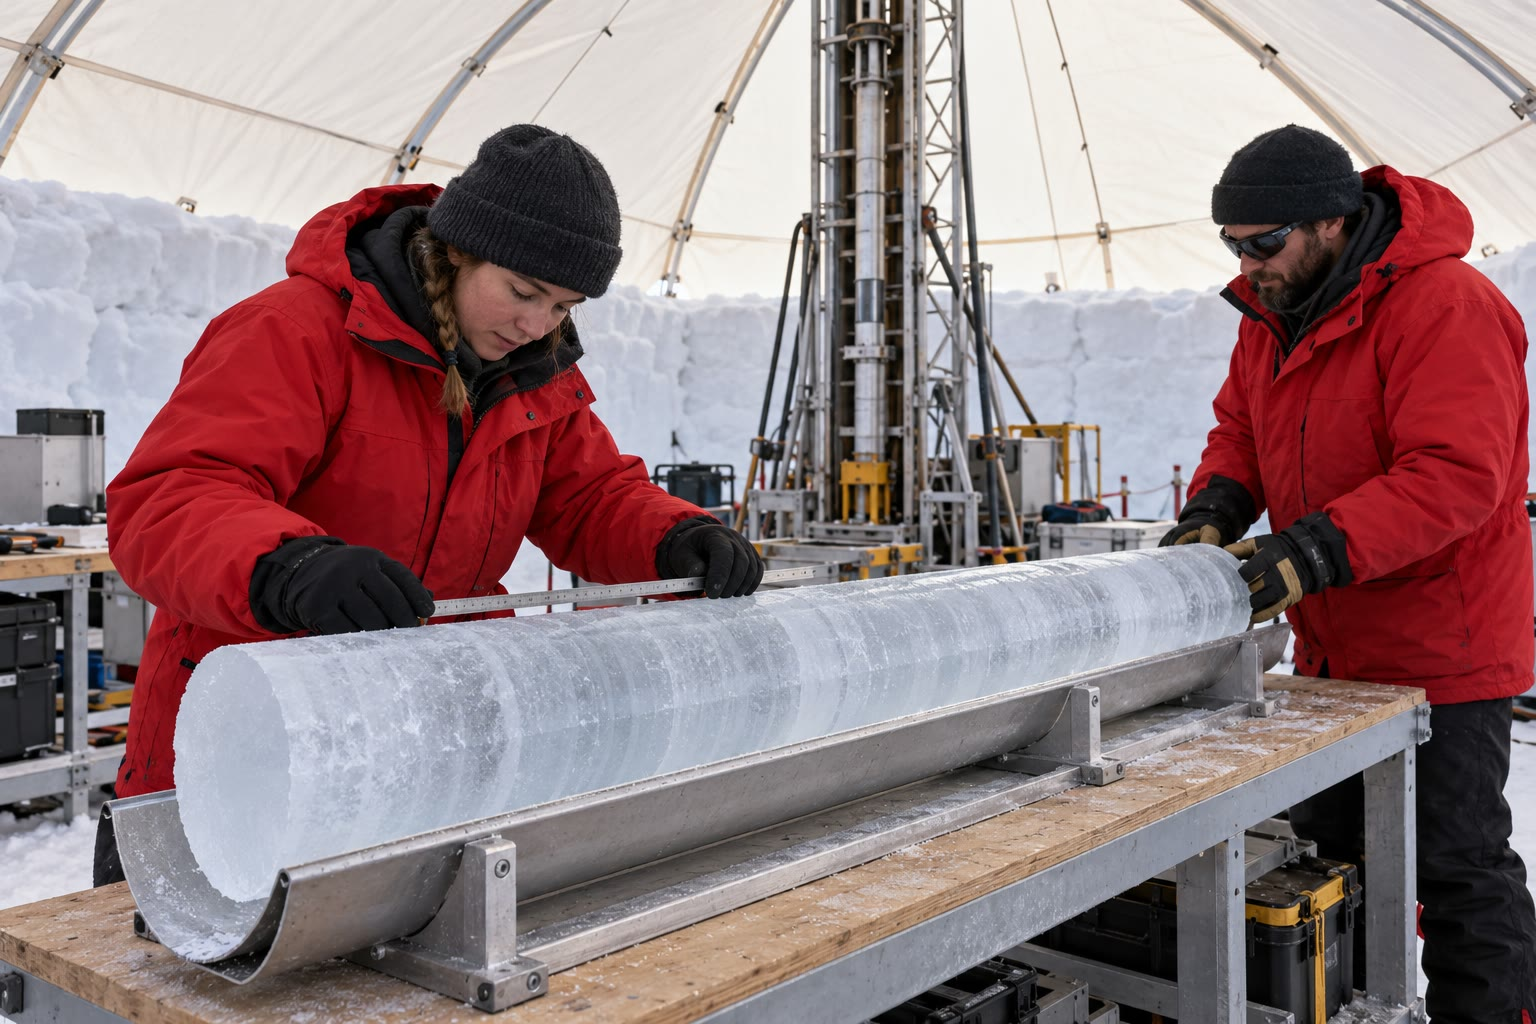
\includegraphics[width=\linewidth]{images/book5/ai/b3-ice-core-tent.jpg}

{\scriptsize हिमचादर पर एक ड्रिलिंग तंबू में पालने में रखे बर्फ़ के कोर को मापा जा रहा है,
पीछे ड्रिल टावर (AI से बनाया गया चित्रण)।}
\end{minipage}
\end{inthelab}

\section{अभ्यास}

\begin{exercise}[$\star$]\label{exo:b3:stable-isotopes:1}
एक कैल्साइट का $\delta^{18}\mathrm O = \qty{30.5}{\permil}$ है, और जिस जल से वह बना उसका
\qty{-2.1}{\permil} है, दोनों VSMOW पर। $\alpha$, $1000\ln\alpha$ और
$\Delta$ परिकलित कीजिए। अंतिम दोनों के बीच कितना अंतर है?
\end{exercise}

\begin{exercise}[$\star$]\label{exo:b3:stable-isotopes:2}
एक उच्च-अक्षांश तटीय स्टेशन का वार्षिक माध्य तापमान
\qty{-25}{\celsius} है। अध्याय के ऐसे स्टेशनों के लिए संबंधों से
उसके वर्षण के $\delta^{18}\mathrm O$, $\delta\mathrm D$ और \omterm{def:b3:stable-isotopes:d-excess}{ड्यूटेरियम आधिक्य} का
पूर्वानुमान लगाइए।
\end{exercise}
% ledger: dansgaard64:effects

\begin{exercise}[$\star$]\label{exo:b3:stable-isotopes:3}
एक बेसिन में कार्बोनेटों का $\delta^{13}\mathrm C = \qty{+1.0}{\permil}$ है और कार्बनिक पदार्थ का
\qty{-26.0}{\permil} है। निवेशों के \qty{-5}{\permil} होने पर,
$f_{\mathrm{org}}$ परिकलित कीजिए।
\end{exercise}
% ledger: planavsky22:forg

\begin{exercise}[$\star$]\label{exo:b3:stable-isotopes:4}
एक ब्रेकियोपॉड खोल का $\Delta_{47} = \qty{0.600}{\permil}$ है।
अध्याय के अंशांकन से ज्ञात कीजिए कि वह किस तापमान पर बना।
\end{exercise}
% ledger: isogeochem:d47

\begin{exercise}[$\star\star$]\label{exo:b3:stable-isotopes:5}
महासागर से वाष्प $\delta^{18}\mathrm O = \qty{-13}{\permil}$ पर निकलती है और
स्थिर $\alpha = 1.0100$ के साथ वर्षा के रूप में झरती है। जब वाष्प
\qty{-33}{\permil} पर पहुँचती है, तब उसका कितना अंश शेष रहता है?
उस समय वर्षा का $\delta^{18}\mathrm O$ क्या है?
\end{exercise}
% ledger: white13c9:rayleigh

\begin{exercise}[$\star\star$]\label{exo:b3:stable-isotopes:6}
\qty{-40}{\permil} पर हिम की तुलना 0 पर के महासागर-जल से कीजिए। उनके बीच $\alpha$,
$1000\ln\alpha$, $1000(\alpha - 1)$ और $\Delta$ परिकलित कीजिए। प्रस्ताव के कौन-से सन्निकटन
विफल होते हैं, और कितने से?
\end{exercise}

\begin{exercise}[$\star\star$]\label{exo:b3:stable-isotopes:7}
एक फ़ोरामिनिफ़ेर का $\delta^{18}\mathrm O = \qty{+1.50}{\permil}$ VPDB है और वह
\qty{0.00}{\permil} VSMOW वाले जल में बना। अध्याय की विधि से
उसका निर्माण-तापमान परिकलित कीजिए, और जल पर \qty{0.1}{\permil} की त्रुटि
उसे कितना बदलती है।
\end{exercise}
% ledger: isogeochem:ko97

\begin{exercise}[$\star\star$]\label{exo:b3:stable-isotopes:8}
बेंथिक स्टैक वर्तमान से अंतिम हिमनदीय अधिकतम तक \qty{1.77}{\permil} बदलता है।
अध्याय में परिकलित हिम-आयतन का अंश हटाइए और शेष को
गहरे-जल के तापमान परिवर्तन में बदलिए, \qty{2}{\celsius} के आसपास के
कैल्साइट अंशांकन की ढलान का उपयोग करते हुए।
\end{exercise}
% ledger: data:lr04, white13c9:ice-volume, isogeochem:ko97

\begin{exercise}[$\star\star$]\label{exo:b3:stable-isotopes:9}
एक पाइराइट का $\delta^{34}\mathrm S = \qty{10.0}{\permil}$ और $\delta^{33}\mathrm S =
\qty{8.2}{\permil}$ है। $\Delta^{33}\mathrm S$ परिकलित कीजिए। जब पाइराइट बना, तब
वायुमंडल के बारे में यह क्या बताता है?
\end{exercise}
% ledger: white13c9:s-mif

\begin{exercise}[$\star\star\star$]\label{exo:b3:stable-isotopes:10}
बंद-तंत्र संघनन में वाष्प और बना हुआ सारा संघनित पदार्थ
एक साथ साम्यावस्था में रहते हैं। दिखाइए कि तब वाष्प के लिए $R_v/R_{v,0} = 1/[f +
\alpha(1 - f)]$ होता है, और $f = 0.2$ तथा
$\alpha = 1.01$ के लिए इसकी तुलना \omterm{prop:b3:stable-isotopes:rayleigh-distillation}{रैले आसवन} से कीजिए।
\end{exercise}

\begin{exercise}[$\star\star\star$]\label{exo:b3:stable-isotopes:11}
\qty{2000}{Gt} मीथेन कार्बन के अनुमान से, जो \qty{-60}{\permil} पर है,
विनिमेय कार्बन में \qty{-2.5}{\permil} का परिवर्तन होता है।
$\delta_0 = 0$ लेकर इससे निहित भंडार द्रव्यमान ज्ञात कीजिए। उस द्रव्यमान के साथ
\qty{-25}{\permil} पर कितना कार्बनिक कार्बन वही परिवर्तन देगा?
प्रकाशित परास से तुलना कीजिए।
\end{exercise}
% ledger: dickens11:petm

\begin{exercise}[$\star\star\star$]\label{exo:b3:stable-isotopes:12}
दिखाइए कि शीतलन पथ के साथ $\mathrm d\delta_v/\mathrm dT = (\alpha - 1)(1000 +
\delta_v)\,\mathrm d\ln e_s/\mathrm dT$ होता है। \qty{-20}{\celsius} पर, जहाँ अध्याय के मॉडल की
वाष्प का $\delta^{18}\mathrm O = \qty{-49.1}{\permil}$ है
और उर्ध्वपातन वक्र $\mathrm d\ln e_s/\mathrm dT =
\qty{0.0960}{K^{-1}}$ देता है, यह ढलान परिकलित कीजिए।
\end{exercise}
% ledger: gkinis14:alpha-ice, iapws:melt-subl

\section{समस्या: डोम इल्से तक एक वर्षा-बूँद की यात्रा}

\begin{problem}[{सप्ताहांत समस्या --- एक काल्पनिक यात्रा-मार्ग के साथ हिम के समस्थानिक,
एक पुरा-तापमान और एक कार्बन विचलन}]\label{pb:b3:stable-isotopes:1}
एक वायु राशि एक काल्पनिक हिमचादर के किनारे से \qty{0}{\celsius} पर
वाष्प के साथ निकलती है, जिसका $\delta^{18}\mathrm O = \qty{-20.0}{\permil}$ और $\delta\mathrm D =
\qty{-150}{\permil}$ है, और स्थिर दाब पर अंतर्देशीय यात्रा करते हुए ठंडी होती है।
कोस्ट स्टेशन पर \qty{-10}{\celsius}, मिडवे पर \qty{-20}{\celsius} और डोम इल्से पर
\qty{-30}{\celsius} पर हिम बनता है, जब शेष वाष्प का अंश
$f = 0.425$, $0.169$ और $0.0622$ होता है। अध्याय के हिम-वाष्प प्रभाजन गुणांक लीजिए,
जो प्रत्येक खंड पर
अपने मध्य तापमान के मान पर स्थिर हों।
% ledger: gkinis14:alpha-ice, iapws:melt-subl, dansgaard64:effects, isogeochem:ko97, isogeochem:d47, white13c9:ice-volume, data:lr04, planavsky22:forg, dickens11:petm

\medskip\noindent\textbf{भाग I --- आसवन।}
\begin{enumerate}
\item $\alpha^{18}$ और $\alpha^{\mathrm D}$ को $-5$, $-10$, $-15$, $-20$,
$-25$ और \qty{-30}{\celsius} पर (ऑक्सीजन के लिए पाँच सार्थक अंक, ड्यूटेरियम के लिए चार)
परिकलित कीजिए।
\item कोस्ट पर पहुँचने पर वाष्प का $\delta^{18}\mathrm O$ परिकलित कीजिए।
\item कोस्ट के हिम का वही मान परिकलित कीजिए।
\item मिडवे के लिए दोहराइए ($f$ का खंड-अनुपात $0.169/0.425$ है)।
\item डोम इल्से के लिए दोहराइए।
\item वाष्प के मूल ऑक्सीजन-18 का कितना अंश
डोम इल्से पर अब भी वायु में शेष है?
\end{enumerate}

\medskip\noindent\textbf{भाग II --- तापमान और ड्यूटेरियम।}
\begin{enumerate}[resume]
\item कोस्ट से डोम इल्से तक हिम के $\delta^{18}\mathrm O$ की
संघनन तापमान के सापेक्ष प्रवणता परिकलित कीजिए।
\item ग्रीनलैंड के स्टेशनों का संबंध डोम इल्से के हिम के लिए कौन-सा
माध्य वार्षिक सतही तापमान निर्धारित करेगा? यह
\qty{-30}{\celsius} से भिन्न क्यों हो सकता है?
\item इसी प्रकार तीनों स्टेशनों पर हिम का $\delta\mathrm D$ परिकलित कीजिए।
\item उनका \omterm{def:b3:stable-isotopes:d-excess}{ड्यूटेरियम आधिक्य} परिकलित कीजिए। अंतर्देशीय क्षेत्र में यह कैसे बदलता है?
\item क्या डोम इल्से का हिम उल्कीय जल रेखा पर स्थित है? मॉडल
वह क्या छोड़ देता है जो वास्तविक हिम संरचना में शामिल होता है?
\end{enumerate}

\medskip\noindent\textbf{भाग III --- तट के पास का एक फ़ोरैमिनिफ़ेरा।}
तट के समीप की अवसाद कोर शीर्ष पर बेंथिक फ़ोरैमिनिफ़ेरा का
मान \qty{3.25}{\permil} VPDB और अंतिम हिमनदीय अधिकतम पर \qty{5.02}{\permil} देती है;
आज तल-जल का मान \qty{0.00}{\permil} VSMOW है।
\begin{enumerate}[resume]
\item कैल्साइट अंशांकन के साथ वर्तमान तल-जल का तापमान
परिकलित कीजिए।
\item जल को अपरिवर्तित मानते हुए हिमनदीय तापमान परिकलित कीजिए। क्या
यह परिणाम संभव है?
\item \qty{125}{m} के समुद्र-तल पतन के लिए हिमनदीय जल का संशोधन कीजिए
और पुनः परिकलन कीजिए। तल-जल का हिमनदीय शीतलन कितना है?
\item दोनों तापमानों पर अपेक्षित $\Delta_{47}$ और उनका
अंतर परिकलित कीजिए।
\item \omterm{def:b3:stable-isotopes:clumped}{गुच्छित समस्थानिक} तापमापी को जल के संघटन की आवश्यकता
क्यों नहीं होती?
\end{enumerate}

\medskip\noindent\textbf{भाग IV --- कार्बन विचलन।} कोर में और गहराई पर,
\qty{+0.5}{\permil} वाले कार्बोनेट एक संक्षिप्त
\qty{-3.0}{\permil} के विचलन से बाधित होते हैं।
\begin{enumerate}[resume]
\item विचलन से पहले, $\delta_{\mathrm{in}} = \qty{-5}{\permil}$ और
$\Delta_B = \qty{-28}{\permil}$ के साथ, $f_{\mathrm{org}}$ परिकलित कीजिए।
\item अभ्यास 11 का भंडार लीजिए, जिसमें शून्य पर \qty{46000}{Gt} है। यदि स्रोत
\qty{-60}{\permil} पर मीथेन है, तो विचलन को कितना कार्बन चाहिए?
\item और यदि यह \qty{-25}{\permil} पर कार्बनिक कार्बन है?
\item और यदि यह \qty{-5}{\permil} पर प्रावार का कार्बन है?
\item उसी कोर में कौन-सा प्रेक्षण स्रोतों के बीच
चुनने में सहायक हो सकता है?
\item डोम इल्से पर गिरते हिम का $\delta^{18}\mathrm O$ बताइए।
\end{enumerate}
\end{problem}
